\documentclass{article}
\usepackage[utf8]{inputenc}
\usepackage{geometry}
\usepackage{graphicx}
\usepackage{amsmath}
\usepackage{amsfonts}
\usepackage{amsthm}
\usepackage{amssymb}
\usepackage[most]{tcolorbox}
\usepackage{array}
\usepackage{latexsym}
\usepackage{alltt}
\usepackage{hyperref}
\usepackage{color}
\usepackage{float}
\usepackage{pdfpages}
\usepackage{algpseudocode}
\usepackage{multicol}
\usepackage{multirow}
\usepackage{caption}
\usepackage{xparse}
\usepackage{setspace}
\usepackage{enumitem}
\usepackage{pdflscape}
\usepackage{mathtools}


\geometry
{
  a4paper,
  left=10mm,
  right=10mm,
  top=10mm,
  bottom=15mm,
}

% mybox
\newtcolorbox{mybox}[3][]
{
  colframe = #2!25,
  colback  = #2!10,
  coltitle = #2!20!black,  
  title    = {#3},
  #1,
}

% New environments that use mybox
\newcounter{example}
\newenvironment{example}[1]{\begin{mybox}{green}{\refstepcounter{example}\textbf{Example~\theexample #1}}}{\end{mybox}}

\newenvironment{example_break}[1]{\begin{mybox}[breakable]{green}{\refstepcounter{example}\textbf{Example~\theexample #1}}}{\end{mybox}}

\newcounter{definition}
\newenvironment{definition}[1]{\refstepcounter{definition}\begin{mybox}{blue}{\textbf{Definition~\thedefinition #1}}}{\end{mybox}}

\newcounter{theorem}
\newenvironment{theorem}[1]{\begin{mybox}{red}{\refstepcounter{theorem}\textbf{Theorem~\thetheorem #1}}}{\end{mybox}}

\newenvironment{formula}[1]{\begin{mybox}{cyan}{\textbf{#1}}}{\end{mybox}}

% Changing maketitle
\makeatletter         
\renewcommand\maketitle{
{\raggedright % Note the extra {
\begin{center}
{\Large \bfseries \@title}\\[2ex] 
{\large \@author \ - \@date}\\[2ex]
\end{center}}} % Note the extra }
\makeatother

% \onehalfspacing % adjust spacing

% macros
\newcommand{\prob}[1]{\textbf{\textit{P}}\{#1\}}
\newcommand{\ra}{\rightarrow}
\newcommand{\Ra}{\Rightarrow}
\newcommand{\xRaL}{\xRightarrow[]{L}}
\newcommand{\vdashm}{\vdash_M^*}
\NewDocumentCommand{\dsum}{%
    e{^_}
}{%
  {% 
    \displaystyle\sum
    \IfValueT{#1}{^{#1}}
    \IfValueT{#2}{_{#2}}
  }
}%

% maketitle variables
\title{CENG 280 - Chapter 3: Context Free Grammer}
\author{Burak Metehan Tunçel}
\date{May, June 2022}

\begin{document}

\maketitle

% \section{Context Free Grammars}

\begin{multicols*}{2}
\setlength{\columnsep}{1.5cm}
\setlength{\columnseprule}{0.2pt}

\begin{itemize}
  \item \textbf{Language Recognizer:} A device that accepts valid strings. For example, finite automata are language recognizer.
  \item \textbf{Language Generator:} A device that generates valid strings.
\end{itemize}

We shall study certain types of formal language generators. Such a device begins, when given some sort of ``start'' signal, to construct a string. Its operation is \textit{not completely determined from the beginning but is nevertheless limited by a set of rules}. Eventually this process halts, and the device outputs a completed string. \textit{The language defined by the device is the set of all strings that it can produce.}

Neither a recognizer nor a generator for the English language is at all easy
to produce. Nevertheless, the idea of a language generator has some explanatory force in attempts to discuss human language. More important for us, however, is \textit{the theory of generators of formal}, ``artificial'' languages, such as the regular languages and the important class of ``context-free'' languages will be introduced.

This theory will neatly \textit{complement the study of automata}, which recognize languages, and is also of practical value in the specification and analysis of computer languages.\\

Regular expressions can be viewed as language generators. 

\noindent For example, consider the regular expression $a(a^* \cup b^*)b$.A verbal description of how to generate a string in accordance with this expression would be the following
\begin{itemize}
  \item First output an $a$. Then do one of the following two things:
  \item Either output a number of $a$'s or output a number of $b$'s.
  \item Finally output a $b$
\end{itemize}
The language associated with this language generator -that is, the set of
all strings that can be produced by the process just described- is, of course, exactly the regular language defined in the way described earlier by the regular expression $a(a^* \cup b^*)b$. 

We will study certain more complex sorts of language generators, called \textbf{context-free grammars}, which are based on a more complete understanding of the structure of the strings belonging to the language.


To take again the example of the language generated by $a(a^* \cup b^*)b$. If we let $S$ be a new symbol interpreted as ``\textit{a string in the language}'', and $M$ be a symbol standing for ``\textit{middle part}'', then we can express this observation by writing
\begin{equation*}
  S \to aMb
\end{equation*}
where $\to$ is read ``\textit{can be}''. We call such an expression a \textbf{rule}. What can $M$, the middle part, be? The answer is: either a string of $a$'s or a string of $b$'s.

\vspace*{\fill}
\columnbreak

\noindent We express this by adding the rules
\begin{align*}
  M \to A \textnormal{    and    } M \to B
\end{align*}
where $A$ and $B$ are new symbols that stand for strings of $a$'s and $b$'s, respectively. Now, what is a string of $a$'s? It can be the empty string
\begin{equation*}
  A \to e
\end{equation*}
or it may consist of a leading a followed by a string of $a$'s:
\begin{equation*}
  A \to aA
\end{equation*}
Similarly, for $B$:
\begin{equation*}
  B \to e \textnormal{    and    } B \to bB
\end{equation*}
The language denoted by the regular expression $a(a^* \cup b^*)b$ can then be defined alternatively by the following language generator.
\begin{quote}
  Start with the string consisting of the single symbol $S$. Find a symbol in the current string that appears to the left of $\to$ in one of the rules above. Replace an occurrence of this symbol with the string that appears to the right of $\to$ in the same rule. Repeat this process until no such symbol can be found.
\end{quote}

For example, to generate the string $aaab$ we start with $S$, as specified; we then replace $S$ by $aMb$ according to the first rule, $S \to aMb$. To $aMb$ we apply the rule $M \to A$ and obtain $aAb$. We then twice apply the rule $A \to aA$ to get the string $aaaAb$. Finally, we apply the rule $A \to e$. In the resulting string, $aaab$, we cannot identify any symbol that appears to the left of $\to$ in some rule. Thus the operation of our language generator has ended, and $aaab$ was produced, as promised.

A \textbf{context-free grammar} is a language generator that operates like the one above, with some such set of rules. Let us pause to explain at this point \textit{why such a language generator is called context-free}. Consider the string $aaAb$, which was an intermediate stage in the generation of $aaab$. It is natural to call the strings $aa$ and $b$ that surround the symbol $A$ the \textbf{context of $A$} in this particular
string. Now, the rule $A \to aA$ says that we can replace $A$ by the string $aA$ no matter what the surrounding strings are; in other words, \textit{independently of the context of $A$}.

In a context-free grammar, some symbols appear to the left of $\to$ in rules -$S$, $M$, $A$, and $B$ in our example- and some -$a$ and $b$- do not. Symbols of the latter kind are called \textbf{terminals}, since the production of a string consisting solely of such symbols signals the termination of the generation process. All these ideas can be stated formally.
\end{multicols*}

\begin{definition}{}
  A \textbf{context-free grammar} $G$ is a quadruple $(V, \Sigma, R, S)$ where
  \begin{itemize}
    \item $V$ is an alphabet
    \item $\Sigma$ (the set of \textbf{terminals}) is a subset of $V$
    \item $R$ (the set of \textbf{rules}) is a finite subset of $(V - \Sigma) \times V^*$
    \item $S$ (the \textbf{start symbol}) is an element of $V - \Sigma$
  \end{itemize}
  The members of $V - \Sigma$ are called \textbf{nonterminals}. For any $A \in V - \Sigma$ and $u \in V^*$, we write $A \rightarrow_G u$ whenever $(A, u) \in R$. For any strings $u, v \in V^*$, we write $u \Rightarrow_G v$ if and only if there are strings $x, y \in V^*$ and $A \in V - \Sigma$ such that $u = xAy$, $v = xv'y$, and $A \rightarrow_G v'$. The relation $\Rightarrow_G^*$ is the \textit{reflexive}, \textit{transitive closure} of $\Rightarrow_G$. Finally, $L(G)$, the \textbf{language generated} by $G$, is $\left\{ w \in \Sigma^* : S \Rightarrow_G^* w \right\}$; we also say that $G$ \textbf{generates} each string in $L(G)$. A language $L$ is said to be a \textbf{context-free language} if $L = L(G)$ for some context-free grammar $G$.
\end{definition}

\noindent When the grammar to which we refer is obvious, we write $A \to w$ and $u \Rightarrow v$ instead of $A \to_G w$ and $u \Rightarrow_G v$.

We call any sequence of the form
\begin{equation*}
  w_0 \Rightarrow_G w_1 \Rightarrow_G \cdots \Rightarrow_G w_n
\end{equation*}
a \textbf{derivation} in $G$ of $w_n$ from $w_0$. Here $w_o, \cdots, w_n$ may be any strings in $V^*$, and $n$, the \textbf{length} of the derivation, may be any natural number, including zero. We also say that the derivation has $n$ \textbf{steps}. 

\begin{example_break}{}
  Consider the context-free grammar $G = (V, \Sigma, R, S)$, where
  \begin{itemize}
    \item $V = \{ S, a, b \}$
    \item $\Sigma = \{ a, b \}$
    \item $R$ consists of the rules $S \to aSb$ and $S \to e$.
  \end{itemize}
  A possible derivation is
  \begin{equation*}
    S \Rightarrow aSb \Rightarrow aaSbb \Rightarrow aabb.
  \end{equation*}
  Here the first two steps used the rule $S \to aSb$, and the last used the rule $S \to e$. In fact, it is not hard to see that $L(G) = \{ a^nb^n\ |\ n \geq 2 \}$. \textit{Hence some context-free languages are not regular, but all regular languages are context-free.}
\end{example_break}

\begin{example_break}{}
  Let $G$ be the grammar $(W, \Sigma, R, S)$, where
  \begin{align*}
    W = \{& S, A, N, V, P \} \cup \Sigma\\
    \Sigma = \{& \textnormal{Jim, big, green, cheese, ate} \}\\
    R = \{& P \to N,\\
          & P \to AP,\\
          & S \to PVP,\\
          & A \to \textnormal{big},\\
          & A \to \textnormal{green},\\
          & N \to \textnormal{cheese},\\
          & N \to \textnormal{Jim},\\
          & V \to \textnormal{ate} \}
  \end{align*}
  Here $G$ is designed to be a grammar for a part of English; $S$ stands for \textit{sentence}, $A$ for \textit{adjective}, $N$ for \textit{noun}, $V$ for \textit{verb}, and $P$ for \textit{phrase}. The following are some strings in $L(G)$.
  \begin{itemize}
    \item Jim ate cheese
    \item big Jim ate green cheese
    \item big cheese ate Jim
  \end{itemize}
  Unfortunately, the following are also strings in $L(G)$:
  \begin{itemize}
    \item big cheese ate green green big green big cheese
    \item green Jim ate green big Jim     
  \end{itemize}
\end{example_break}

\noindent \textbf{\textit{Note:}} \textit{Example 3.1.3, 3.1.4 and 3.1.5 should be read from book.}

\begin{formula}{}
  \begin{itemize}
    \item $u \Rightarrow v$: $u$ \textbf{\textit{directly yields}} $v$; $A \rightarrow w$: \textbf{\textit{(production) rule}}.
    \item $V$, alphabet, can include symbols such as start symbol, $S$, or $A$.
    \item (From example 3.1.4) The same string may have several derivations in a context-free grammar. Two derivations in this grammar are
    \begin{align*}
      &S \Rightarrow SS \Rightarrow S(S) \Rightarrow S((S)) \Rightarrow S(()) \Rightarrow ()(()) &\textnormal{ and } && S \Rightarrow SS \Rightarrow (S)S \Rightarrow ()S \Rightarrow ()(S) \Rightarrow ()(())
    \end{align*}
    \item Some context-free languages are not regular. However, all regular languages are context-free.
    \item Context-free languages are precisely the languages accepted by certain language acceptors called \textit{\textbf{pushdown automata}}.
  \end{itemize}
\end{formula}

\begin{figure}[h]
  \centering
  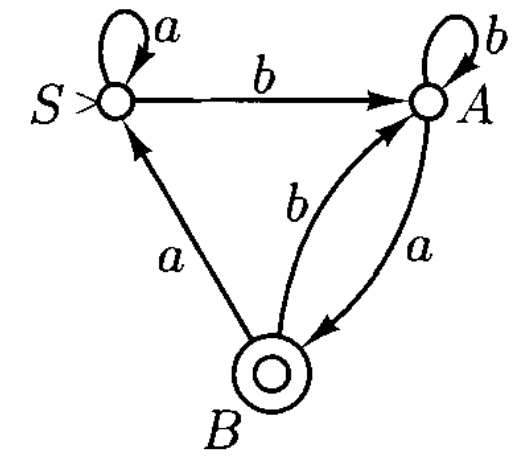
\includegraphics[width=.2\textwidth]{img/fig3-1.png}
  \caption{}
\end{figure}

\begin{proof}
  We can prove the statement ``\textit{all regular languages are context-free}'' by a \textit{\textbf{direct construction}}. Consider the regular language accepted by the deterministic finite automaton $M = (K, \Sigma, \delta, s, F)$. The same language is generated by the grammar $G(M) = (V, \Sigma, R, S)$, where $V = K \cup \Sigma$, $S = s$, and $R$ consists of these rules:
  \begin{equation*}
    R = \left\{ q \to ap\ |\ \delta(q, a) = p \right\} \cup \left\{ q \to e\ |\ q \in F \right\}
  \end{equation*}
  That is, the nonterminals are the states of the automaton; as for rules, for each transition from $q$ to $p$ on input $a$ we have in $R$ the rule $q \to p$. For example, for the automaton in Figure 1 we would construct this grammar:
  \begin{equation*}
    S \to aS,\ S \to bA,\ A \to aB,\ A \to bA,\ B \to aS,\ B \to bA,\ B \to e.
  \end{equation*}
\end{proof}


% \section{Parse Trees}

\begin{multicols}{2}
\setlength{\columnsep}{1.5cm}
\setlength{\columnseprule}{0.2pt}

Let $G$ be a context-free grammar. A string $w \in L(G)$ may have many derivations in $G$. For example, if $G$ is the context-free grammar that generates the language of balanced parentheses, then the string $()()$ can
be derived from $S$ by at least two distinct derivations, namely,
\begin{equation*}
    S \Rightarrow SS \Ra (S)S \Ra ()S \Ra ()(S) \Ra ()()
\end{equation*}
and
\begin{equation*}
    S \Rightarrow SS \Ra S(S) \Ra (S)(S) \Ra (S)() \Ra ()()
\end{equation*}
However, these two derivations are in a sense ``the same''. The rules used are the same, and they are applied at the same places in the intermediate string. The only difference is in the order in which the rules are applied. Intuitively, both derivations can be pictured as in Figure 2.
\begin{figure}[H]
    \centering
    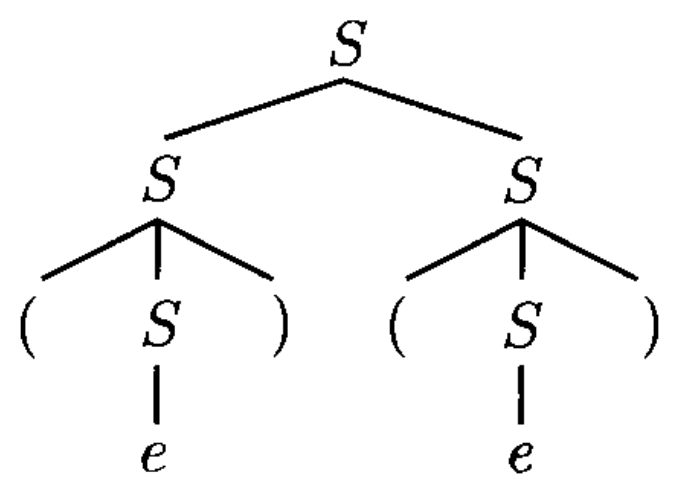
\includegraphics[width=.2\textwidth]{img/fig3-2.png}
    \caption{}
\end{figure}

We call such a picture a \textbf{parse tree}. The points are called \textbf{nodes}; each node carries a \textbf{label} that is a symbol in $V$. The topmost node is called the \textbf{root}, and the nodes along the bottom are called \textbf{leaves}. All leaves are labeled by \textit{terminals}, or possibly the empty string $e$. By concatenating the labels of the leaves from left to right, we obtain the derived string of terminals, which is
called the \textbf{yield} of the parse tree.

%% Add definition after drawing with tikz

More formally, for an arbitrary context-free grammar $G = (V, \Sigma, R, S)$, we define its parse trees and their roots, leaves, and yields, as follows.

\begin{enumerate}
    \item
        \begin{equation*}
            \circ\ a
        \end{equation*}
        This is a parse tree for each $a \in \Sigma$. The single node of this parse tree is both the root and a leaf. The yield of this parse tree is $a$.
    
    \item If $A \ra e$ is a rule in $R$, then % Later draw with tikz
        \begin{figure}[H]
            \centering
            
\includegraphics[width=.4\textwidth]{img/parse-tree-2.png}
        \end{figure}
        is a parse tree; its root is the node labeled $A$, its sole leaf is the node labeled $e$, and its yield is $e$.
    
    \item If
        \begin{figure}[H]
            \centering
            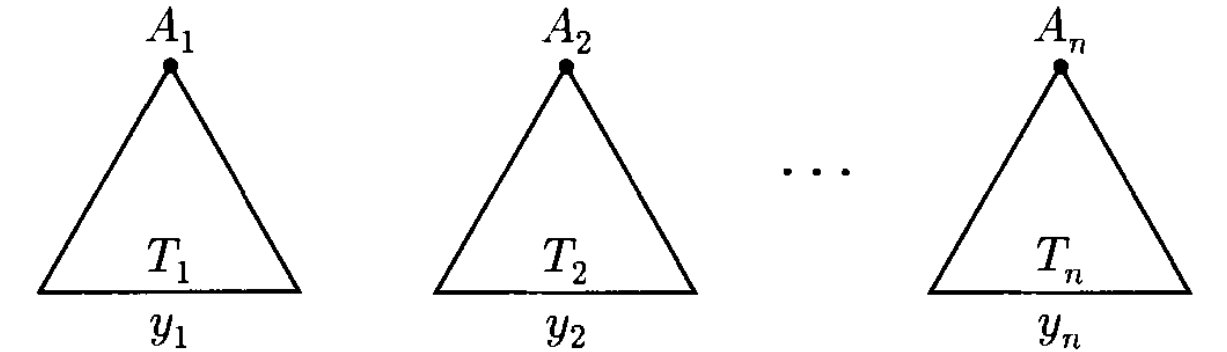
\includegraphics[width=.4\textwidth]{img/parse-tree-3.png}
        \end{figure}
        are parse trees, where $n > 1$, with roots labeled $A_1, \ldots, A_n$ respectively, and with yields $y_1, \ldots, y_n$, and $A \ra A_1 \ldots A_n$ is a rule in $R$, then
        \begin{figure}[H]
            \centering
            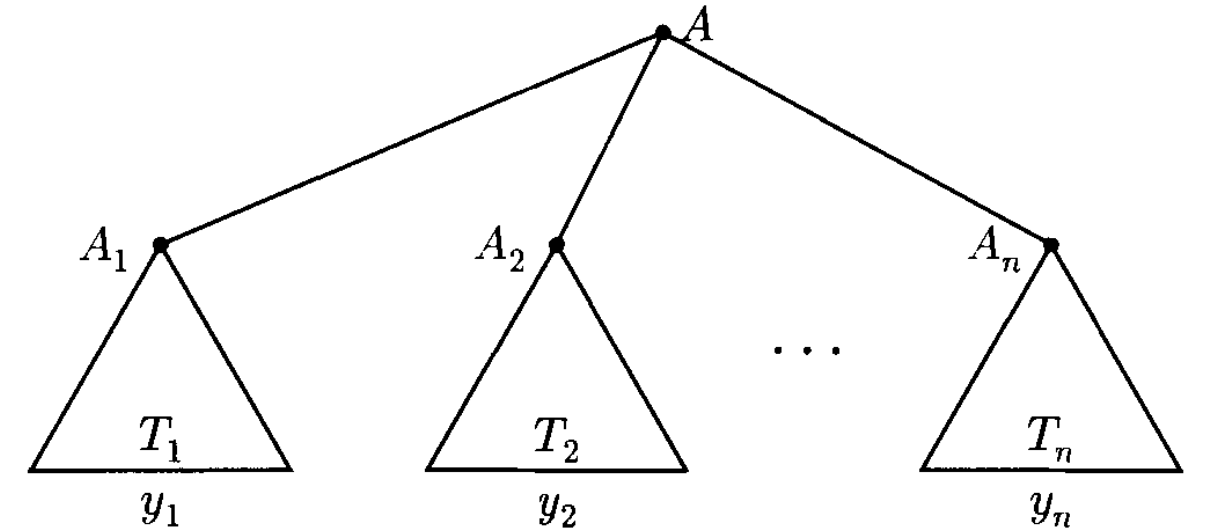
\includegraphics[width=.4\textwidth]{img/parse-tree-4.png}
        \end{figure}
        is a parse tree. Its root is the new node labeled $A$, its leaves are the leaves of its constituent parse trees, and its yield is $y_1 \ldots y_n$.
    
    \item Nothing else is a parse tree.
\end{enumerate}

Intuitively, parse trees are ways of representing derivations (\textit{the process of deriving a string}) of strings in $L(G)$ so that the superficial differences between derivations, owing to the order of application of rules, are suppressed. To put it otherwise, parse trees represent
equivalence classes of derivations. We make this intuition precise below. 

Let $G = (V, \Sigma, R, S)$ be a context-free grammar, and let $D = x_1 \Ra x_2 \Ra \cdots \Ra x_n$ and $D' = x_1' \Ra x_2' \Ra \cdots \Ra x_n'$ be two derivations in $G$, where $x_i, x_i' \in V^*$ for $i = 1, \ldots, n$; $x_1, x_1' \in V - \Sigma$; and $x_n, x_n' \in \Sigma^*$. That is, they are both derivations of terminal strings from a single nonterminal. We say that $D$ \textbf{precedes} $D'$, written $D \prec D'$, if $n > 2$ and there is an integer $k$, $1 < k < n$ such that

\begin{enumerate}
    \item for all $i \neq k$ we have $x_i = x_i'$;
    \item $x_{k-1} = x_{k-1}' = uAvBw$, where $u, v, w \in V^*$, and $A, B \in V - \Sigma$;
    \item $x_k = uyvBw$, where $A \ra y \in R$;
    \item $x_k' = uAvzw$, where $B \ra y \in R$;
    \item $x_{k+1} = x_{k+1}' = uyvzw$.
\end{enumerate}

In other words, the two derivations are identical except for two consecutive steps, during which the same two nonterminals are replaced by the same two strings \textit{but in opposite orders in the two derivations}. The derivation in which the leftmost of the two nonterminals is replaced first is said to precede the other.

\end{multicols}

\begin{example}{}
    Consider the following three derivations $D_1$ , $D_2$ , and $D_3$ in the grammar $G$ generating all strings of balanced parentheses:
    \begin{align*}
        D_1 &= S \Ra SS \Ra (S)S \Ra ((S))S \Ra (())S \Ra (())(S) \Ra (())()\\
        D_2 &= S \Ra SS \Ra (S)S \Ra ((S))S \Ra ((S))(S) \Ra (())(S) \Ra (())()\\
        D_3 &= S \Ra SS \Ra (S)S \Ra ((S))S \Ra ((S))(S) \Ra ((S))() \Ra (())()
    \end{align*}
    We have that $D_1 \prec D_2$ and $D_2 \prec D_3$. However, it is not the case that $D_1 \prec D_3$, since the two latter derivations differ in more than one intermediate string. Notice that all three derivations have the same parse tree, the one shown in Figure 3-4

    \begin{figure}[H]
        \centering
        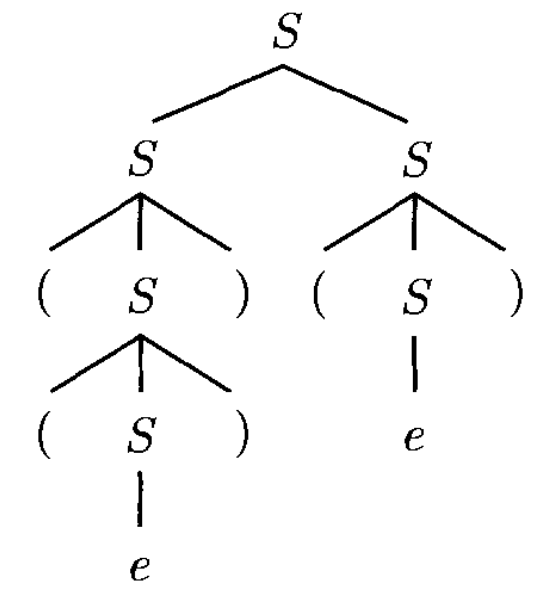
\includegraphics[width=.2\textwidth]{img/fig3-4.png}
        \caption{}
    \end{figure}
\end{example}

\begin{multicols}{2}
\setlength{\columnsep}{1.5cm}
\setlength{\columnseprule}{0.2pt}
    
We say that two derivations $D$ and $D'$ are \textbf{similar} if the pair $(D, D')$ belongs in the \textit{reflexive, symmetric, transitive closure} of $\prec$. Since the reflexive, symmetric, transitive closure of any relation is by definition reflexive, symmetric, and transitive, similarity is an equivalence relation. To put it otherwise, two derivations are similar if they can be transformed into another via a sequence of ``switchings'' in the order in which rules are applied. Such a ``switching'' can replace a derivation either by one that precedes it, or by one that it precedes.

Each equivalence class of derivations under similarity, that is to say, each parse tree, contains a derivation that is \textit{maximal} under $\prec$; that is, it is not preceded by any other derivation. This derivation is called a \textbf{leftmost derivation}. A leftmost derivation exists in every parse tree, and it can be obtained as follows. Starting from the label of the root $A$, repeatedly replace the \textit{leftmost nonterminal in the current string} according to the rule suggested by the parse tree. Similarly, a \textbf{rightmost derivation} is one that does not precede any other derivation; it is obtained from the parse tree by always expanding the \textit{rightmost nonterminal in the current string}. \textit{Each parse tree has exactly one leftmost and exactly one rightmost derivation}. This is so because the leftmost derivation of a parse tree is uniquely determined, since at each step there is one nonterminal to replace: the leftmost one. Similarly for the rightmost derivation.

It is easy to tell when a step of a derivation can be a part of a leftmost derivation: the leftmost nonterminal must be replaced. We write $x \xRightarrow[]{L} y$ if and only if $x = wA\beta$, $y = w\alpha\beta$, where $w \in \Sigma^*$; $\alpha, \beta \in V^*$; $A \in V - \Sigma$; and $A \ra \alpha$ is a rule of $G$. Thus, if $x_1 \Ra x_2 \Ra \cdots \Ra x_n$ is a leftmost derivation, then in fact $x_1 \xRightarrow[]{L} x_2 \xRightarrow[]{L} \cdots \xRightarrow[]{L} x_n$ Similarly for rightmost derivations (the notation is $x \xRightarrow[]{R} y$).

To summarize our insights into parse trees and derivations in this section, we state without formal proof the following theorem.

\begin{theorem}{}
    Let $G = (V, \Sigma, R, S)$ be a context-free grammar, and let $A \in V - \Sigma$, and $w \in \Sigma^*$. Then the following statements are equivalent:
    \begin{itemize}
        \item $A \Ra^* w$.
        \item There is a parse tree with root $A$ and yield $w$.
        \item There is a leftmost derivation $A \xRightarrow[]{L}^* w$.
        \item There is a rightmost derivation $A \xRightarrow[]{R}^* w$. 
    \end{itemize}
\end{theorem}

\subsection{Ambiguity}

There may be a string in the language generated by a context-free grammar with two derivations that are \textit{not similar} -that is to say, with two distinct parse trees, or, equivalently, with two distinct rightmost derivations (and two distinct leftmost derivations).

Given a grammar $G = (V, \Sigma, R, S)$, if a string $w \in L(G)$ has two different parse trees (two different derivations that are not similar), then the grammar is called \textbf{ambiguous}. Assigning a parse tree to a string is called ``\textit{parsing}''. It is an important concept since parsing allows us to understand why the string belongs to the grammar. In addition, it gives a ``\textit{meaning}'' (or \textit{interpretation}) to the string, which is particularly important for the programming languages.

A context-free language $L$ is called \textbf{inherently ambiguous} if every grammar $G$ that generate $L$, i.e. $L = L(G)$, is \textit{ambiguous}.

\end{multicols}


% \section{Pushdown Automata}

Not every context-free language can be recognized by a finite automaton, since some context-free languages are not regular.

To be able to accept the context-free language, an automata needs to have a stack. The idea of an automaton with a stack as auxiliary storage can be formalized as follows. 

\begin{definition}{}
  \textbf{Pushdown automaton} is a sextuple $M = (K, \Sigma, \Gamma, \Delta, s, F)$ where
  \begin{itemize}
    \item $K$ is a finite set of \textbf{states},
    \item $\Sigma$ is an alphabet (\textbf{input symbols})
    \item $\Gamma$ is an alphabet (\textbf{stack symbols})
    \item $s \in K$ is the \textbf{initial state}
    \item $F \subseteq K$ is the set of \textbf{final states}, and,
    \item $\Delta \subset (K \times (\Sigma \cup \{e\}) \times \Gamma^*) \times (K \times \Gamma^*)$ is a finite \textbf{transition relation}.
  \end{itemize}
\end{definition}

If $((p, a, \delta),(q, \gamma)) \in \Delta$, then when $M$ is in state $p$, if it reads $a \in \Sigma$ (or if $a$ is $e$ without reading a symbol) and if the top of the stack is $\delta$, it enters state $q$ and replaces $\delta$ with $\gamma$. $((p, a, \delta),(q, \gamma)) \in \Delta$ is called a \textbf{transition} of $M$. Since $\Delta$ is a relation, several transitions can be applicable at a point. The machine chooses non-deterministically from the applicable transitions.
\begin{itemize}
  \item $((p, a, e),(q, b))$: \textbf{push} transition, read $a$ push $b$ to the top of the stack.
  \item $((p, a, b),(q, e))$: \textbf{pop} transition, read $a$ pop $b$ from the top of the stack.
  \item $((p, a, \delta),(q, \gamma))$: read $a$, \textbf{pop} $\delta$ and \textbf{push} $\gamma$.
\end{itemize}

\newpage
\noindent The \textbf{configuration} of a pushdown automaton is a member of $K \times \Sigma^* \times \Gamma^*$:
\begin{enumerate}
  \item The first component is the \textit{state of the machine},
  \item The second is the \textit{unread part of the input type},
  \item The third is the \textit{contents of the pushdown store, read top-down}.\\
\end{enumerate}

\noindent A configuration $(p, x, \alpha)$ of $M$ yields $(q, y, \zeta)$ (shown as $(p, x, \alpha) \vdash_M (q, y, \zeta))$ if there is a transition $((p, a, \beta),(q, \gamma))$ such that
\begin{center}
  \begin{multicols}{3}
    \begin{enumerate}
      \item $x = ay$
      \item $\alpha = \beta \eta$
      \item $\zeta = \gamma \eta$
    \end{enumerate}
  \end{multicols}
\end{center}
\noindent for some $\eta \in \Gamma^*$. The reflexive transitive closure of $\vdash_M$ is denoted by $\vdash_M^*$. $M$ accepts a word $w \in \Sigma^*$ if and only if $(s, w, e) \vdash_M^* (f, e, e)$ for some $f \in F$. In other words, $M$ accepts $w$ iff there exists a sequence of configurations $C_0, \ldots, C_n$ with $C_0 = (s, w, e)$ and $C_n = (f, e, e)$ for some $f \in F$, and $C_0 \vdash_M C_1 \vdash_M \ldots \vdash_M C_n$. Any sequence $C_0, \ldots, C_n$ with $C_i \vdash_M C_{i+1}$ is called a \textbf{computation} of $M$. It has \textbf{length} $n$ (or $n$ steps). The language accepted by $M$, $L(M)$ is the set of strings accepted by $M$. (When no confusion can result, we write $\vdash$ and $\vdash^*$ instead of $\vdash_M$ and $\vdash_M^*$.)


\section{Pushdown Automata and Context Free Grammars}

\begin{multicols*}{2}
\setlength{\columnsep}{1.5cm}
\setlength{\columnseprule}{0.2pt}

\begin{theorem}{}
\textit{The class of languages accepted by pushdown automata is exactly the class of context-free languages.}
\end{theorem}

\textbf{Proof:} We break this proof into two parts.

\begin{formula}{ Lemma 1}
\textit{Each context-free language is accepted by some pushdown automaton.}
\end{formula}

\begin{proof}
Let $G = (V, \Sigma, R, S)$ be a context-free grammar; we must construct a pushdown automaton $M$ such that ${L(M) = L(G)}$. The machine we construct has only two states, $p$ and $q$, and remains permanently in state $q$ after its first move. Also, $M$ uses $V$, the set of terminals and nonterminals, as its stack alphabet. We let $M = (\{ p, q \}, \Sigma, V, \Delta, p, \{ q \})$, where $\Delta$ contains the following transitions:
\begin{enumerate}
  \item $((p, e, e),\ (q, S))$
  \item $((q, e, A),\ (q, x))$ for each rule $A \ra x$ in $R$.
  \item $((q, a, a),\ (q, e))$ for each $a \in \Sigma$.
\end{enumerate}
The pushdown automaton $M$ begins by pushing $S$, the start symbol of $G$, on its initially empty pushdown store, and entering state $q$ (transition 1). On each subsequent step, it either replaces the topmost symbol $A$ on the stack provided that it is a nonterminal, by the right-hand side $x$ of some rule $A \ra x$ in $R$ (transitions of type 2), or pops the topmost symbol from the stack, provided that it is a terminal symbol that matches the next input symbol (transitions of type 3). 

The transitions of $M$ are designed so that the pushdown store during an accepting computation mimics a leftmost derivation of the input string.

To continue the proof of the Lemma, in order to establish that $L(M) = L(G)$, we prove the following claim

\begin{quote}
\textbf{Claim:} Let $w \in \Sigma^*$ and ${\alpha \in (V - \Sigma)V^* \cup \{ e \}}$. Then ${S \xRightarrow[]{L}^* w\alpha}$ iff ${(q, w, S) \vdash_M^* (q, e, \alpha)}$.
\end{quote}
This claim will suffice to establish Lemma 1, since it will follow (by taking $\alpha = e$) that $S \xRightarrow[]{L}^* w$ if and only if $(q, e, S) \vdash_M^* (q, e, e)$ in other words, $w \in L(G)$ if and only if $w \in L(M)$.

(\textit{Only if}) Suppose that $S \xRightarrow[]{L}^* w\alpha$, where $w \in \Sigma^*$, and $\alpha \in (V - \Sigma)V^* \cup \{ e \}$. We shall show by induction on the length of the leftmost derivation of $w$ from $S$ that $(q, w, S) \vdash_M^* (q, e, \alpha)$.

\noindent \textit{Basis Step}. If the derivation is of length 0, then $w = e$, and $\alpha = S$, and hence indeed $(q, w, S) \vdash_M^* (q, e, \alpha)$.

\noindent \textit{Induction Hypothesis}. Assume that if $S \xRightarrow[]{L}^* w\alpha$ by a derivation of length $n$ or less, $n \geq 0$, then $(q, w, S) \vdash_M^* (q, e, \alpha)$.

\noindent \textit{Induction Step}. Let
\begin{equation*}
  S = u_0 \xRaL u_1 \xRaL \cdots \xRaL u_n \xRaL u_{n+1} = w\alpha
\end{equation*}
be a leftmost derivation of $w\alpha$ from $S$. Let $A$ be the leftmost nonterminal of $u_n$. Then $u_n = xA\beta$, and $u_{n+1} = x\gamma\beta$ where $x \in \Sigma^*$, $\beta$, $\gamma \in V^*$, and $A \ra \gamma$ is a rule in $R$. Since there is a leftmost derivation of length $n$ of $u_n = xA\beta$ from $S$, by the induction hypothesis
\begin{equation}
  (q, x, S) \vdashm (q, e, A\beta)
\end{equation}
Since $A \ra \gamma$ is a rule in $R$,
\begin{equation}
  (q, e, A\beta) \vdash (q, e, \gamma\beta)
\end{equation}
by a transition of type 2.

Now notice that $u_{n+1}$ is $w\alpha$, but it is also $x\gamma\beta$. Hence, there is a string $y \in \Sigma^*$ such that $w = xy$ and $y\alpha = \gamma\beta$. Thus, we can rewrite (1) and (2) above as
\begin{equation}
  (q, w, S) \vdashm (q, y, \gamma\beta)
\end{equation}
However, since $y\alpha = \gamma\beta$
\begin{equation}
  (q, y, \gamma\beta) \vdashm (q, e, \alpha)
\end{equation}
by a sequence of $|y|$ transitions of type 3. Combining (3) and (4) completes the induction step. 

(\textit{If}) Now suppose that $(q, w, S) \vdashm (q, e, \alpha)$ with $w \in \Sigma^*$ and $\alpha \in (V - \Sigma)V^* \cup \{ e \}$; we show that $S \xRaL w\alpha$. Again, the proof is by induction, but this time on the number of transitions of type 2 in the computation by $M$.

\textit{Basis Step}. Since the first move in any computation is by a transition of type 2, if $(q, w, S) \vdashm (q, e, \alpha)$ with no type-2 transitions, then $w = e$ and $\alpha = S$, and the result is true.

\textit{Induction Hypothesis}. If $(q, w, S) \vdashm (q, e, \alpha)$ by a computation with $n$ type 2 steps or fewer, $n \geq 0$, then $S \xRaL w\alpha$.

\textit{Induction Step}. Suppose that $(q, w, S) \vdashm (q, e, \alpha)$ in $n + 1$ type-2 transitions, and consider the next-to-Iast such transition, say,
\begin{equation*}
  (q, w, S) \vdashm (q, y, A\beta) \vdash (q, y, \gamma\beta) \vdashm (q, e, \alpha)
\end{equation*}
where $w = xy$ for some $x, y \in \Sigma^*$, and $A \ra \gamma$, is a rule of the grammar. By the induction hypothesis we have that $S \xRaL xA\beta$, and thus $S \xRaL x\gamma\beta$. Since however $(q, y, \gamma\beta) \vdashm (q, e, \alpha)$, presumably by transitions of type 3, it follows that $y\alpha = \gamma\beta$, and thus $S \xRaL xy\alpha = w\alpha$. This completes the proof of Lemma 1, and with it half the proof of Theorem 2.
\end{proof}

We now turn to the proof of the other half of Theorem 2.

\begin{formula}{ Lemma 2}
\textit{If a language is accepted by a pushdown automaton, it is a context-free language.}
\end{formula}

\begin{proof}
  It will be helpful to restrict somewhat the pushdown automata under consideration. Call a pushdown automaton \textbf{simple} if the following is true:
  \begin{quote}
    Whenever $(( q,\ a,\ \beta),\ (p,\ \gamma))$ is a transition of the pushdown automaton and $q$ is not the start state, then $\beta \in \Gamma$, and $|\gamma| \leq 2$.
  \end{quote}
  In other words, the machine always consults its topmost stack symbol (and no symbols below it), and replaces it either with $e$, or with a single stack symbol, or with two stack symbols. Now it is easy to see that no interesting pushdown automaton can have only transitions of this kind, because then it would not be able to operate when the stack is empty (for example, it would not be able to start the computation, since in the beginning the stack is empty). This is why we do not restrict transitions from the start state.

  We claim that if a language is accepted by an unrestricted pushdown automaton, then it is accepted by a simple pushdown automaton. To see this, let $M = (K,\ \Sigma,\ \Gamma,\ \Delta,\ s,\ F)$ be any pushdown automaton; we shall construct a simple pushdown automaton $M' = (K',\ \Sigma,\ \Gamma \cup \{ Z \},\ \Delta',\ s',\ \{ f \})$ that also accepts $L(M)$; here $s'$ and $f'$ are new states not in $K$, and $Z$ is a new stack symbol, the stack \textit{bottom symbol}, also not in $\Gamma$. We first add to $\Delta$ the transition $(( s',\ e,\ e),\ (s,\ Z))$; this transition starts the computation by placing the stack bottom symbol in the bottom of the stack, where it will remain throughout the computation. No rule of $\Delta'$ will ever push a $Z$ in the stack - except to replace it at the bottom of the stack. We also add to $\Delta'$ the transitions $((f,\ e,\ Z),\ (f',\ e))$ for each $f \in F$. These transitions end the computation by removing $Z$ from the bottom of the
  stack and accepting the input seen so far.

  Initially, $\Delta'$ consists of the start and final transitions described above, and all transitions of $\Delta$. We shall next replace all transitions in $\Delta'$ that violate the simplicity condition by equivalent transitions that satisfy the simplicity condition. We shall do this in three stages:
  \begin{itemize}
    \item First we shall replace transitions with $|\beta| \geq 2$.
    \item Then we shall get rid of transitions with $|\gamma| > 2$, without introducing any transitions with $|\beta| \geq 2$.
    \item Finally, we shall get rid of transitions with $\beta = e$, without introducing any transitions with $|\beta| \geq 2$ or $|\gamma| > 2$.
  \end{itemize}

  
\end{proof}





\end{multicols*}

\end{document}
